%%==================================================================%%
%% Author : Tejedo Gonz�lez, Daniel                                 %%
%%          S�nchez Barreiro, Pablo                                 %%
%% Version: 1.0, 18/11/2012                                         %%                   %%                                                                  %%
%% Memoria del Proyecto Fin de Carrera                              %%
%% Antecedentes, emftext                                      %%
%%==================================================================%%


EMFText es una herramienta espec�ficamente dise�ada para dise�ar las gram�ticas de los lenguajes que hayan sido dise�ados previamente con un metamodelo de Ecore. Est� especializado para la creaci�n de Lenguajes Espec�ficos de Dominio, aunque tambi�n se pueden crear lenguajes de prop�sito general. 

Pero, como en casi todos los casos de este tipo de herramientas, su mayor virtud es la enorme cantidad de c�digo autogenerado que produce, y que elimina al programador de tareas tediosas que adem�s en muchos casos podr�an resultar complicadas. Todo el c�digo generado es completamente independiente de EMFText, es decir, podr� ser ejecutado en plataformas que no tengan la herramienta instalada. 

Todo el c�digo generado por EMFText est� dise�ado de tal modo que sea f�cil de modificar en caso de que queramos poner en pr�ctica algunas funcionalidades poco habituales. Se facilita mucho la labor a la hora de modificar estructuras como el postprocesador de nuestra gram�tica. Todas las gram�ticas construidas tendr�n que ser LL por defecto, a no ser que queramos modificar los parsers generados, posibilidad tambi�n disponible. 

Otro tipo de funcionalidades implementadas, quiz�s no tan importantes pero tambi�n de gran utilidad, son el coloreado de c�digo (por defecto o personalizable), funci�n de completar c�digo, generaci�n del �rbol parseado en el la vista de eclipse Outline o generaci�n de c�digo para crear un depurador para nuestro lenguaje.

\begin{figure}[t]
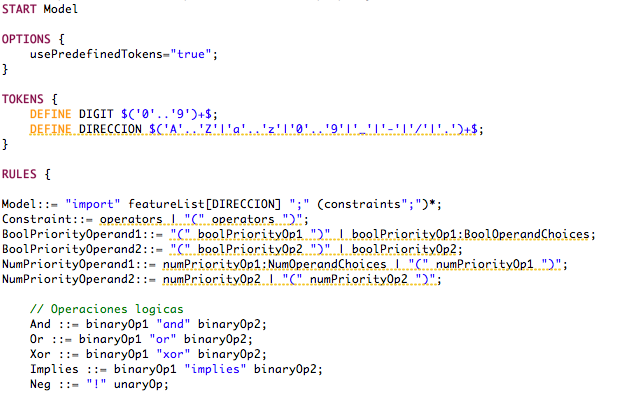
\includegraphics[scale=0.5]{background/gramatica.jpg}
\caption{Trozo de la gram�tica de nuestro editor de especificaci�n y validaci�n de restricciones}
\label{fig5}
\end{figure}


EMFText permite la definici�n de gram�ticas utilizando un lenguaje est�ndar para la definici�n de expresiones regulares, adem�s de incorporar algunas particularidades propias que facilitan ciertas tareas. En la figura \ref{fig5} se muestra una peque�a captura que contiene una porci�n de la gram�tica construida para nuestro editor de especificaci�n y validaci�n de restricciones. 